\section{Subsistema: Localização e Informações}
	Este tópico descreve as soluções para localização do veículo no terreno da lavoura, sua trajetória e
	como serão processados e armazenados os dados coletados das medições.

  \subsection{Sensoriamento: Localização}

  \subsubsection{Ultrassom (HC-SR04)}

Considerando a necessidade de informações referentes à distância com a finalidade de auxiliar a orientação e navegação autônoma do veículo conforme as rotinas estabelecidas pelo algoritmo “\textit{Wall Follower}”, que será discutido detalhadamente, foram discutidos modelos de sensores de distância capazes de preencher os requisitos de navegação.  Inicialmente havia-se optado por um sensor baseado em infravermelho, a partir do princípio de triangulação. Posteriormente essa opção não foi validada devido ao caráter binário do sensor. Sendo assim, foi iniciada uma nova busca, e por fim, foi escolhido o sensor de distância ultrassônico HC-SR04.

		\begin{figure}[!htbp]
			\begin{center}
				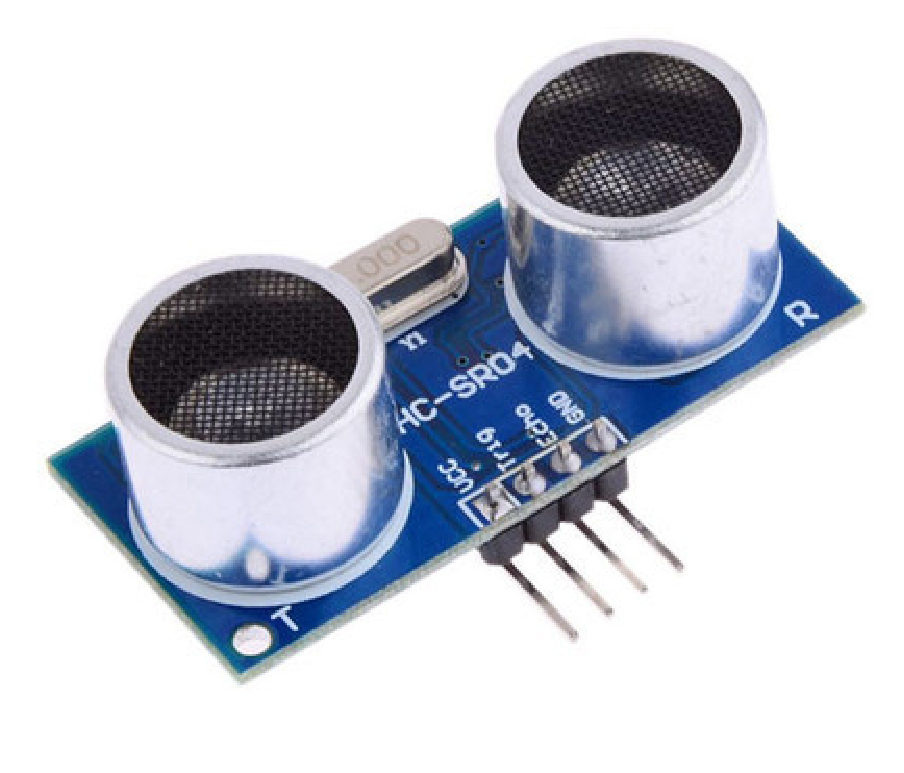
\includegraphics[width=.4\textwidth]{figuras/hcsr04.eps}
				\caption{HC-SR04}
			\end{center}
		\end{figure}

O princípio de funcionamento dos sensores ultrassônicos está baseado na emissão de uma onda sonora de alta frequência, e na medição do tempo levado para a recepção do eco produzido quando esta onda se choca com um objeto capaz de refletir o som.
A detecção do eco incidente, depende de sua intensidade e esta da distância entre o objeto e o sensor ultrassônico. Os sensores ultrassônicos funcionam medindo o tempo de propagação do eco. Isto é, o intervalo de tempo medido entre o impulso sonoro emitido e o eco do mesmo conforme a figura abaixo.
A construção do sensor faz com que o feixe ultrassônico seja emitido em forma cônica.

	\begin{figure}[!htbp]
		\begin{center}
			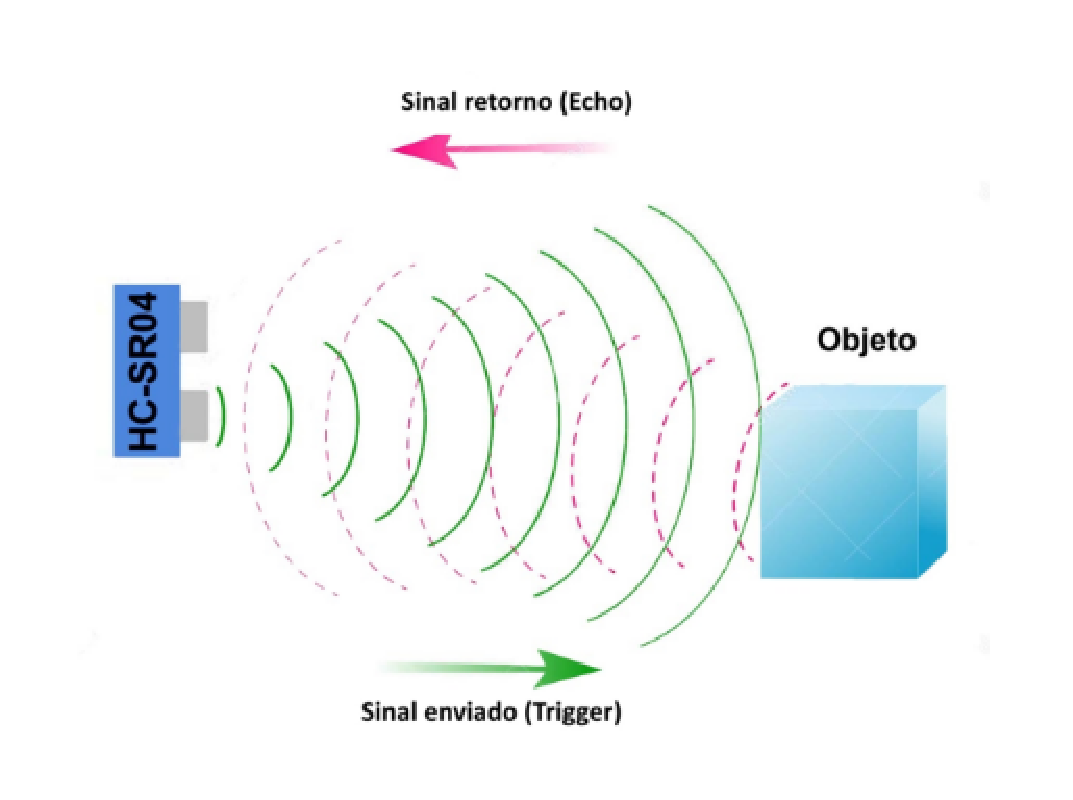
\includegraphics[width=.7\textwidth]{figuras/echo.eps}
			\caption{Sinais de envio e retorno}
		\end{center}
	\end{figure}

O HC-SR04 foi escolhido por apresentar um alcance de 2cm a 4m com uma precisão de 3mm, apresenta uma tensão de operação de 5V, e um ângulo de efeito de 15$^{\circ}$. Seu funcionamento é baseado no envio de um pulso de 10$\mu$s, indicando o início da transmissão de dados. Depois disso, são enviados 8 pulsos de 40 KHz e o sensor aguarda o retorno, para determinar a distância entre o sensor e o objeto, utilizando a equação seguinte:

$$
\textrm{Distância} = \frac{\textrm{Tempo echo em nível alto} \times \textrm{Velocidade do som}}{2}
$$

	\begin{figure}[!htbp]
		\begin{center}
			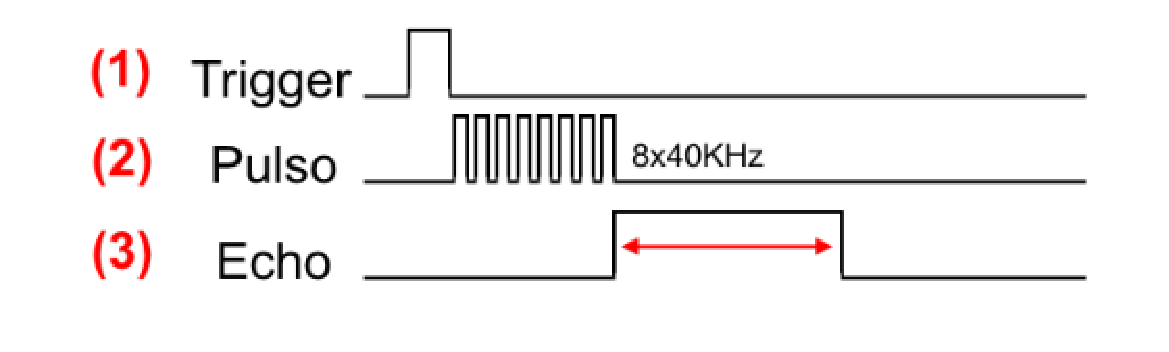
\includegraphics[width=.7\textwidth]{figuras/hcsr04_signals.eps}
			\caption{Sinais de envio e retorno}
		\end{center}
	\end{figure}

\paragraph{Implementação}
Sua implementação foi realizada utilizando a biblioteca aberta \texttt{Ultrasonic.h}.
Além disso, as ligações entre o sensor e o microcontrolador foram realizadas conforme a figura~\ref{fig:hcsr04test}.

	\begin{figure}[!htbp]
		\begin{center}
			\includegraphics[width=.7\textwidth]{figuras/ultrasonic_test.eps}
			\caption{\label{hcsr04test}Circuito implementado.}
		\end{center}
	\end{figure}

	\paragraph{Testes}

	\begin{figure}[!htbp]
	\begin{center}
	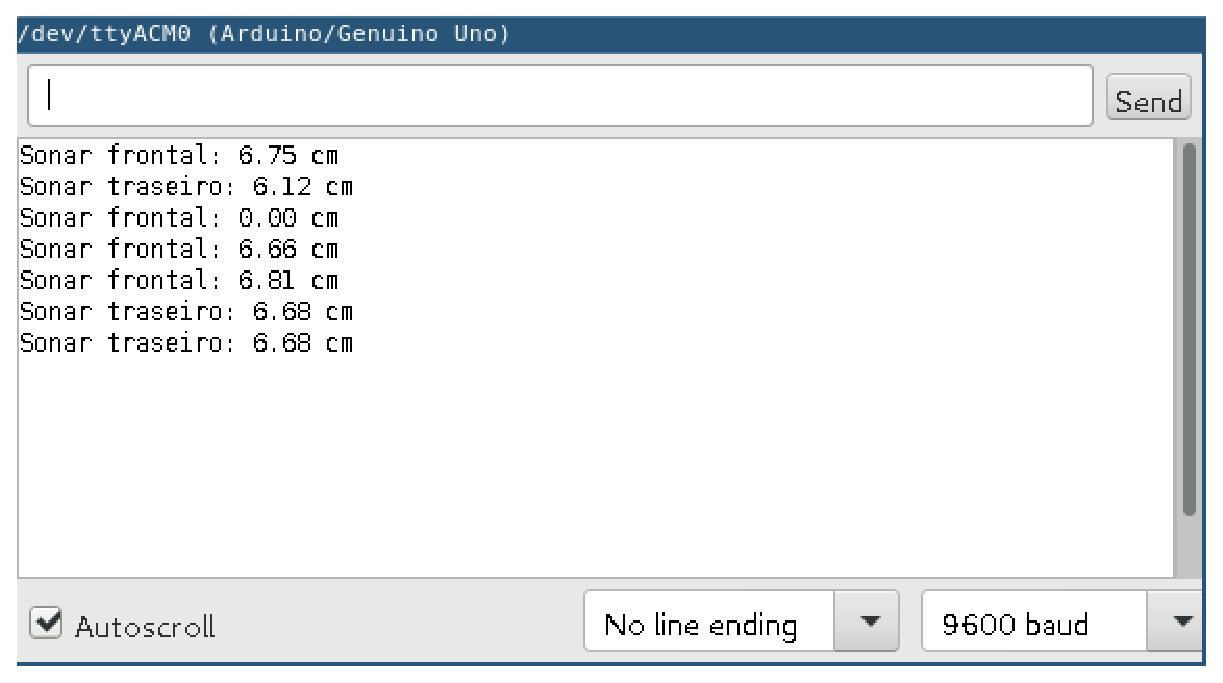
\includegraphics[width=.7\textwidth]{figuras/hcsr04_arduino.eps}
	\caption{\label{fig:hcsr04ardu}Aquisição dos dados dos sensores ultrassônicos com o microcontrolador.}
	\end{center}
	\end{figure}

	\begin{figure}[!htbp]
	\begin{center}
	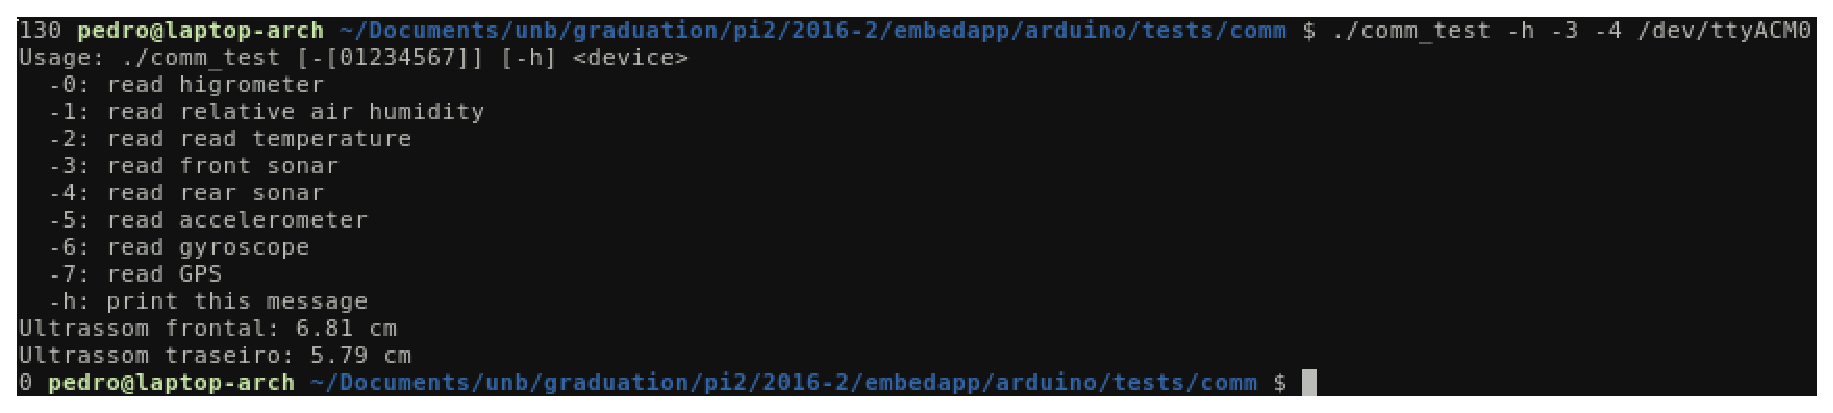
\includegraphics[width=\textwidth]{figuras/hcsr04_raspberry.eps}
	\caption{\label{fig:hcsr04rasp}Aquisição dos dados dos sensores ultrassônicos pela Raspberry Pi.}
	\end{center}
	\end{figure}


  \subsection{Algoritmo de Locomoção}
    Dado a utilização de sensores de ultrassom e a disposição da lavoura de morango
    é possível identificar um típico problema denominado \textit{Wall Follower}.

    Segundo \cite{huang2009}, \textit{Wall Follower},
    também conhecido como regra da mão direita ou esquerda, é válido para percursos conexos, onde todas as paredes são ligadas entre si, mantendo a mão próxima a parede do labirinto em
    que se inclui, garantindo assim que o corpo não se perca e finalize
    o percurso. O principal problema desta regra ocorre quando um percurso
    possui loops de passagens que projetem uma trajetória sem fim.

    \begin{figure}[!htbp]
    \begin{center}
    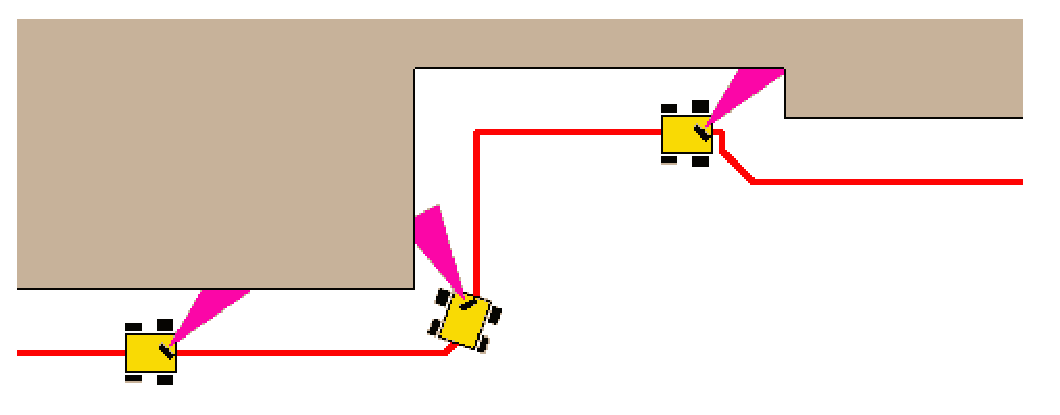
\includegraphics[width=.7\textwidth]{figuras/wallfollower.eps}
    \caption{\label{fig:wallfollower}Exemplo de \textit{Wall Follower}.}
    \end{center}
    \end{figure}

    \vfill
    \pagebreak

    Basicamente o veículo utilizará as paredes dos canteiros como guia, realizando a
    coleta de dados sempre a sua direita. Para viabilizar essa solução serão necessárias algumas adaptações no terreno com a adição de estruturas à lavoura, criando uma espécie de circuito. A figura \ref{fig:ambientadapt} representa o caminho a ser seguido pelo veículo.

    \begin{figure}[!htbp]
    \begin{center}
    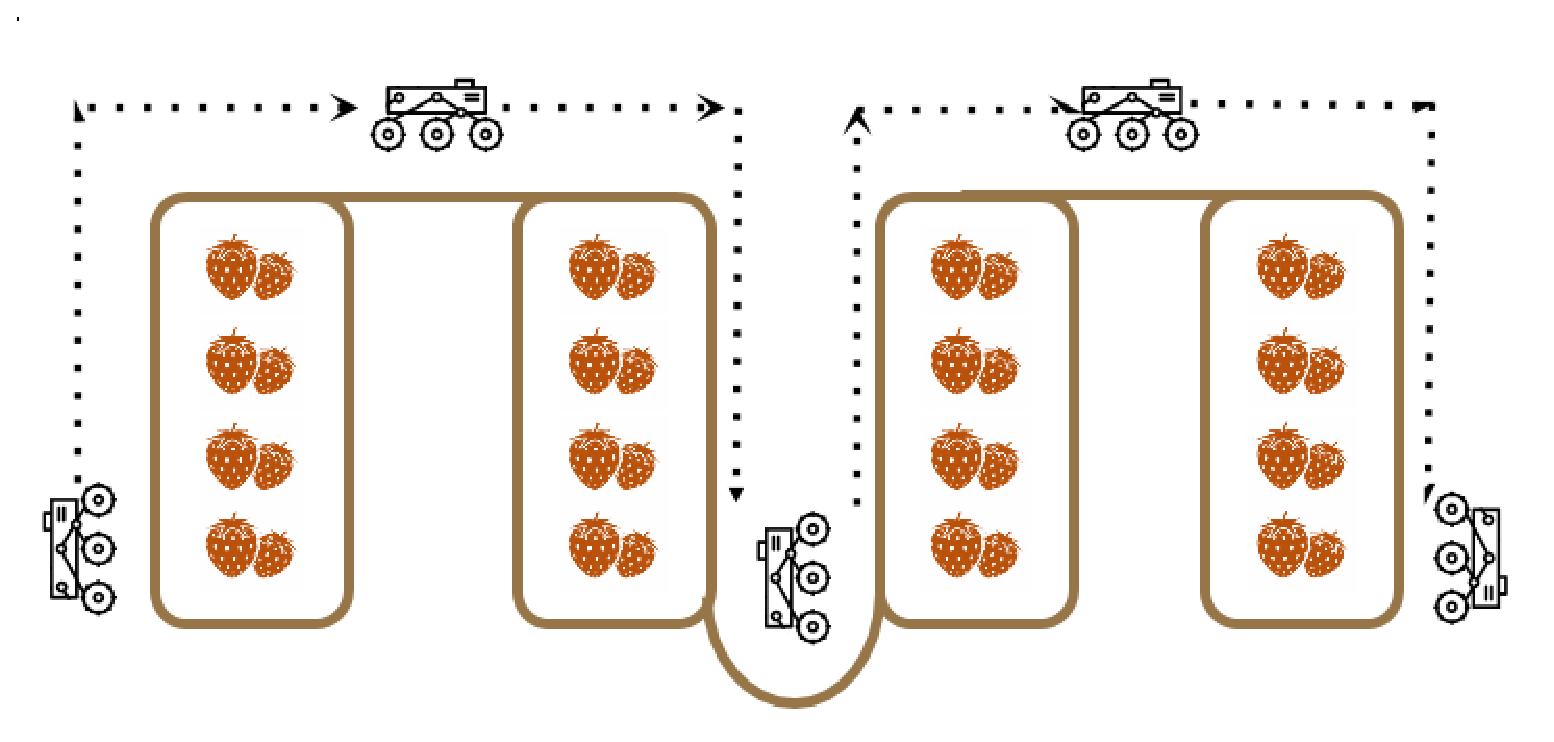
\includegraphics[width=.7\textwidth]{figuras/adapt.eps}
    \caption{\label{fig:ambientadapt}Adaptação do ambiente.}
    \end{center}
    \end{figure}

    \vfill
    \pagebreak

    Para a escolha dos componentes para a construção das barreiras ponderou-se
    necessidade de um material barato e de fácil instalação/manuseio.
    Desta forma, o plástico e a madeira foram os materiais escolhidos para compor os obstáculos
    que irão ajudar o veículo a percorrer o trajeto.

  \subsection{Máquina de Estados para \textit{Wall Follower}}
  Para a execução do código que fará com que o carrinho não colida na parede, elaborou-se uma máquina de estados para que os dois sensores de ultrassom interajam entre si.

  O primeiro estado será responsável por acionar os sensores e enviar o comando para que eles coletem os dados.

  De acordo com os dados coletados pelos sensores, o próximo processo será uma função que realizará o cálculo para medição distância que cada sensor estará da parede definida.

  Inicialmente estabeleceram-se 3 distâncias para que cada sensor ultrassônico defina em que posição ele estará, sabendo-se que haverá um sensor (S1) na parte frontal e outro (S2) na parte traseira do veículo e que a parede de referência será a parede da direita.

  Assim definiu-se três posições para cada sensor, perto, meio, longe. Tendo em vista essas definições, o carrinho poderá estar posicionado em nove diferentes posições possíveis, como ilustra a Tabela \ref{tab:state_wall_follower}.

  \begin{table}[!htbp]
  \centering
  \caption{Tabela de Estados \textit{Wall Follower}}
  \label{tab:state_wall_follower}
  \begin{tabular}{|c|c|c|}
  \hline
  Distância Sensor S1 & Distância Sensor S2 & Estado \\ \hline
  Perto               & Perto                & Left- \\ \hline
  Perto               & Meio                 & Left  \\ \hline
  Perto               & Longe                & Left+ \\ \hline
  Meio                & Perto               & Right  \\ \hline
  Meio                & Meio                & D.N.   \\ \hline
  Meio                & Longe               & Left   \\ \hline
  Longe               & Longe               & Right- \\ \hline
  Longe               & Meio                & Right  \\ \hline
  Longe               & Perto              & Right+  \\ \hline
  \end{tabular}
  \end{table}

  A partir das posições que o veículo poderá estar, deverá se mover em um determinado ângulo para que volte ao centro do caminho e não se choque em nenhuma parede. Então foi definido 7 estados para a execução do \textit{wall follower}: \textit{Left}-, \textit{Left}, \textit{Left}+, D.N.(Do nothing), \textit{Right}-, \textit{Right}, \textit{Right}+. Cada estado enviará um comando ao servo motor para que ele vire em um determinado ângulo:
  \begin{itemize}
    \item \textit{Left}-: envia um comando ao servo motor (motor que muda a direção) para ir à esquerda suavemente, pois o carrinho não está muito virado para a direita, porém está próximo da parede direita;
    \item \textit{Left}: envia um comando ao servo motor para virar à esquerda moderadamente, pois o carrinho está levemente virado para a direita, logo ele tem que virar pra esquerda com mais urgência;
    \item \textit{Left}+: envia um comando ao servo motor para virar à esquerdo, porém com a maior angulação possível, devido o veículo estar quase perpendicular à parede;
    \item \textit{Do Nothing} (D.N.): nesse estado o veículo está a posição desejada para continuar seguido reto, logo não será necessário virar para nenhum lado;
    \item \textit{Right}-: estado em que o veículo deverá virar moderadamente para a direita, pois ele está paralelo a parede, porém perto da parede esquerda;
    \item \textit{Right}: envia um sinal ao servo motor para que ele vire para a direita mais que o “\textit{Right}-“;
    \item \textit{Right}+: esse estado o veículo estará virado para a esquerda quase perpendicular à parede, precisando virar o máximo para a direita, para que volte a posição correta.
  \end{itemize}

  \subsection{Solução Algoritmo}
  O algoritmo de locomoção do veículo, figura \ref{fig:main_algoritmo}, foi escrito em linguagem C e utiliza como base os valores referentes
  ao total de canteiros, quantidade de medições por canteiro e distância entre as medições, os quais
  encontram-se em um arquivo denominado "\textit{settings.conf}". Inicialmente são lidos e armazenados tais valores
  em três variáveis, logo em seguida é lido o nome do \textit{device driver} que realizará a comunicação com o Arduino (argumento passado quando o programa é executado). Tendo conhecimento desse \textit{device driver} é iniciado uma UART que possibilita a comunicação do programa em C com o Arduino, ou seja, a possibilidade de ler dados dos sensores e enviar comandos que o Arduino irá realizar. É chamado o método \textit{start\_navigation} que irá tratar todo o resto do percurso e ao fim do mesmo é fechado o arquivo \textit{settings.conf} e finalizada a UART.

  \begin{figure}[!htbp]
  \begin{center}
  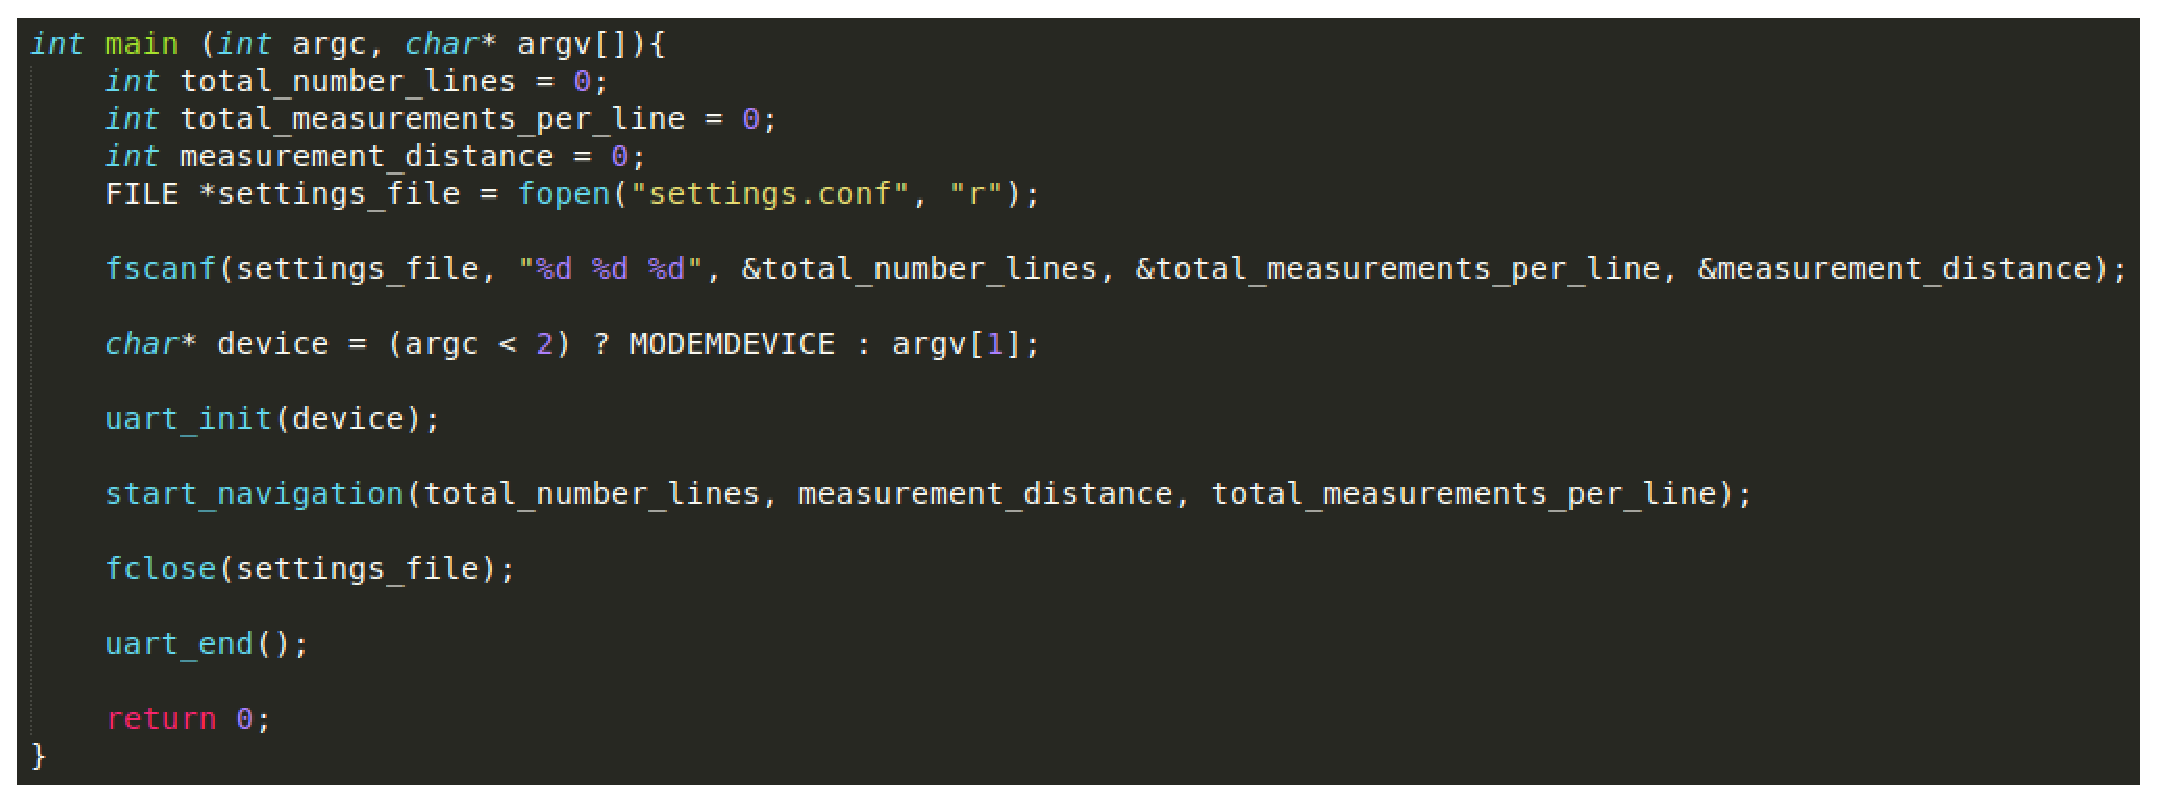
\includegraphics[width=1\textwidth]{figuras/main.eps}
  \caption{\label{fig:main_algoritmo}Início Algoritmo de Locomoção.}
  \end{center}
  \end{figure}

  Tendo conhecimento do percurso que o veículo percorrerá, figura \ref{fig:ambientadapt}, definiu-se que os eventos realizados pelo veículo serão:
  \begin{itemize}
    \item Realizar coleta de dados de um canteiro;
    \item Realizar primeira curva à direita;
    \item Realizar segunda curva à direita;
    \item Realizar novamente coleta de dados de um canteiro;
    \item Realizar curva maior.
  \end{itemize}

  Na figura \ref{fig:start_navigation} encontra-se o corpo do método \textit{start\_navigation}, o qual
  é responsável por executar, em sequência, os eventos citados anteriormente até que o circuito
  seja devidamente concluído (número de canteiros analisados igual ao número total de canteiros).

  \begin{figure}[!htbp]
  \begin{center}
  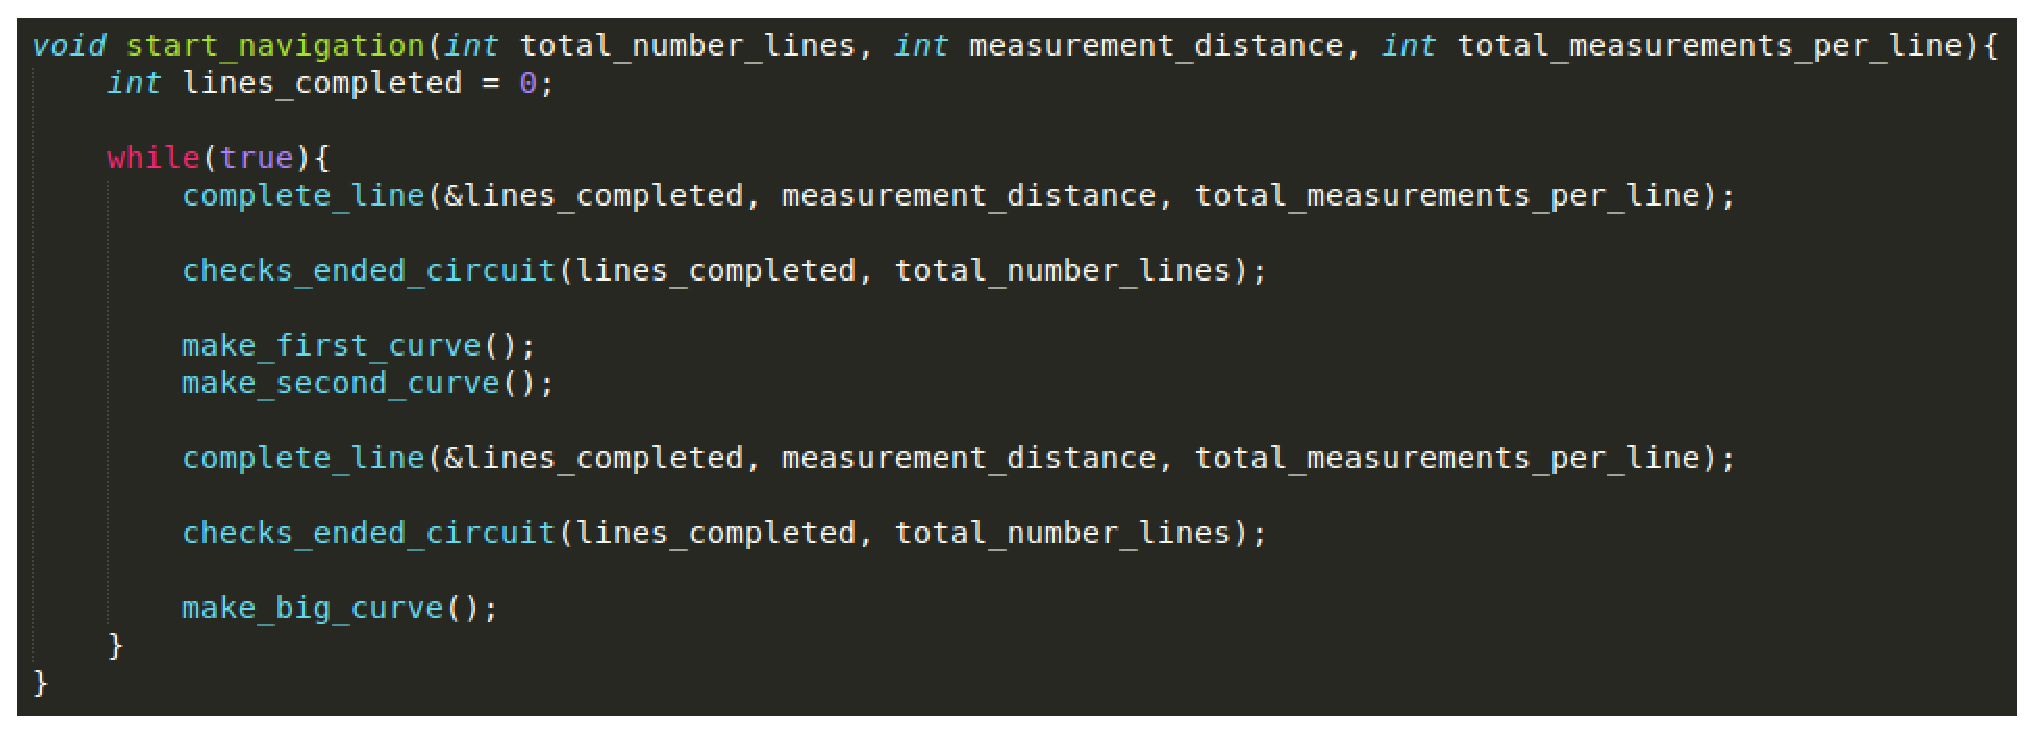
\includegraphics[width=1\textwidth]{figuras/start_navigation.eps}
  \caption{\label{fig:start_navigation}Corpo do Método \textit{start\_navigation}.}
  \end{center}
  \end{figure}

  A função \textit{complete\_line}, figura \ref{fig:complete_line}, é responsável por verificar a distância percorrida pelo veículo, mantê-lo
  seguro em relação à parede e realizar a coleta de dados referentes a um canteiro. A parte de verificação
  da distância percorrida pelo veículo ainda está em desenvolvimento, porém, a mesma partirá do princípio
  de iniciar um timer, coletar a velocidade instantânea do veículo e calcular a distância que foi percorrida.
  Após o veículo locomover-se a distância necessária para uma medição, que
  será realizada através da função \textit{start\_drill}, o processo se repetirá até que todas as medições da fileira sejam atingidas. Ao final desse processo, o número de canteiros medidos será incrementado em uma unidade.

  \begin{figure}[!htbp]
  \begin{center}
  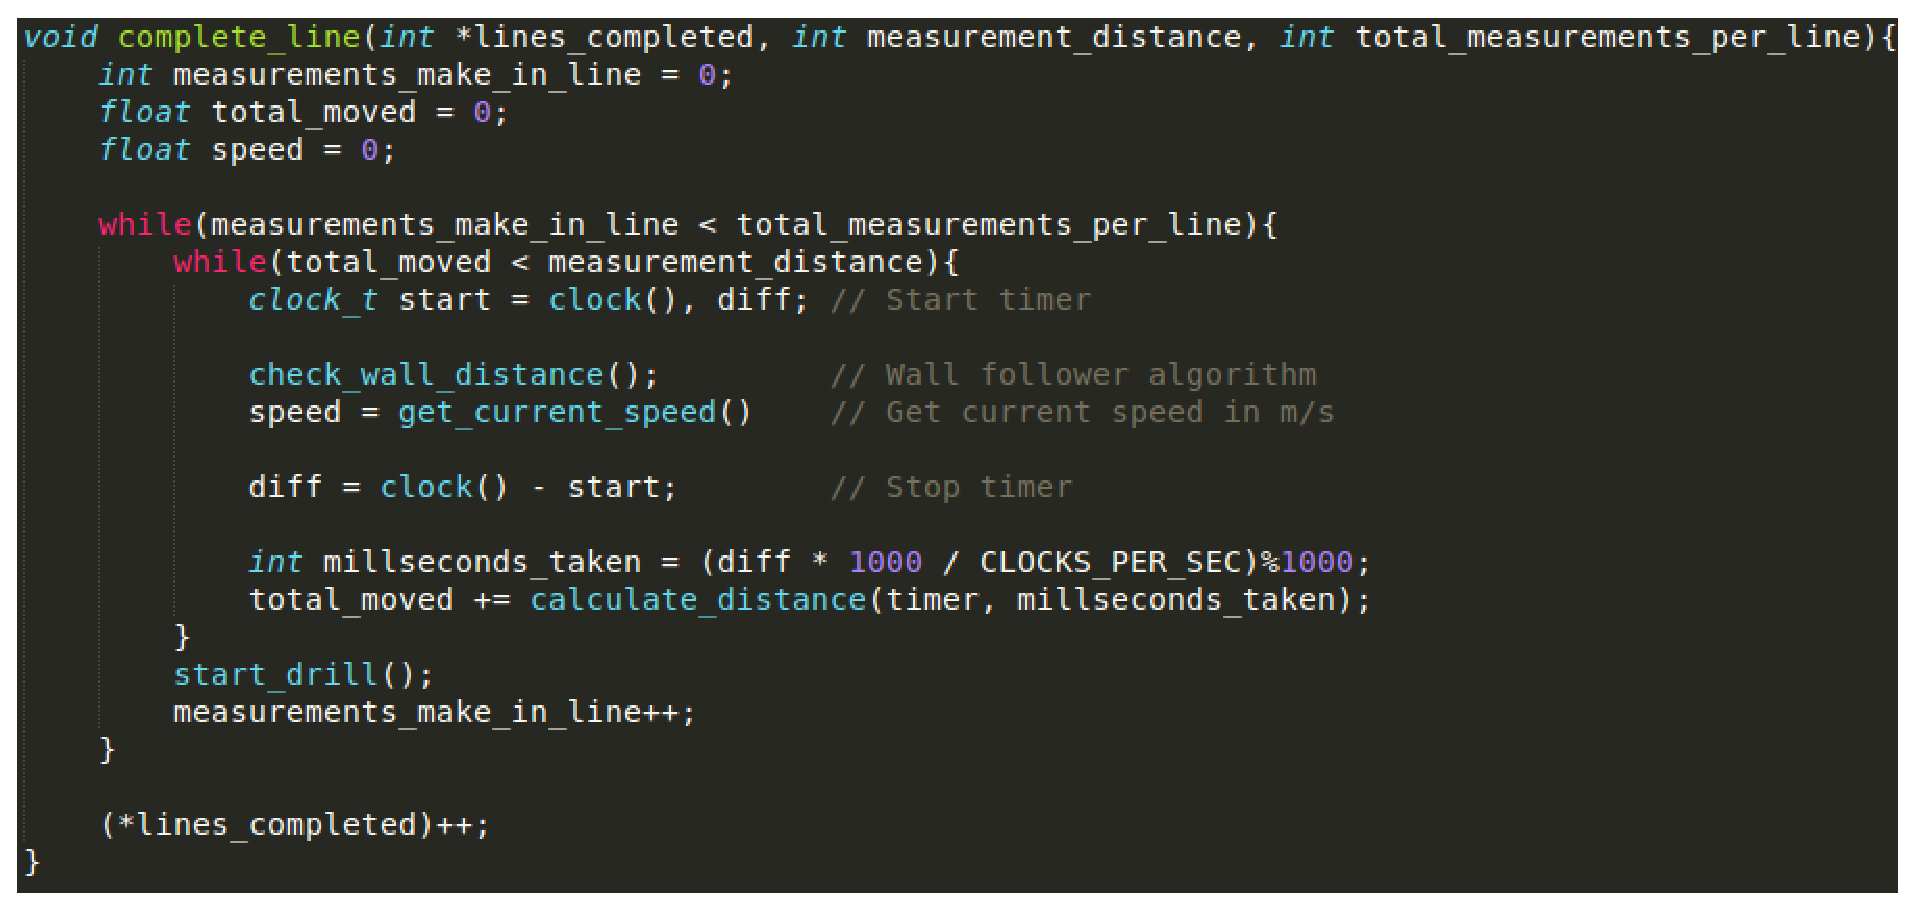
\includegraphics[width=1\textwidth]{figuras/complete_line.eps}
  \caption{\label{fig:complete_line}Corpo do Método \textit{complete\_line}.}
  \end{center}
  \end{figure}

  O princípio do algoritmo de \textit{Wall Follower} encontra-se no método \textit{check\_wall\_distance}, figura \ref{fig:check_wall_distance}, uma vez que são lidos os dados dos sensores ultrassônicos com auxílio
  da função \textit{read\_sonar} e verificado em qual estado o veículo encontra-se, assim, com base nesse estado, será chamada uma função que irá direcionar o veículo para uma distância segura. Como a função de direcionamento do veículo ainda não foi implementada, apenas é imprimido na tela a distância de cada um dos sensores ultrassônicos.

  \begin{figure}[!htbp]
  \begin{center}
  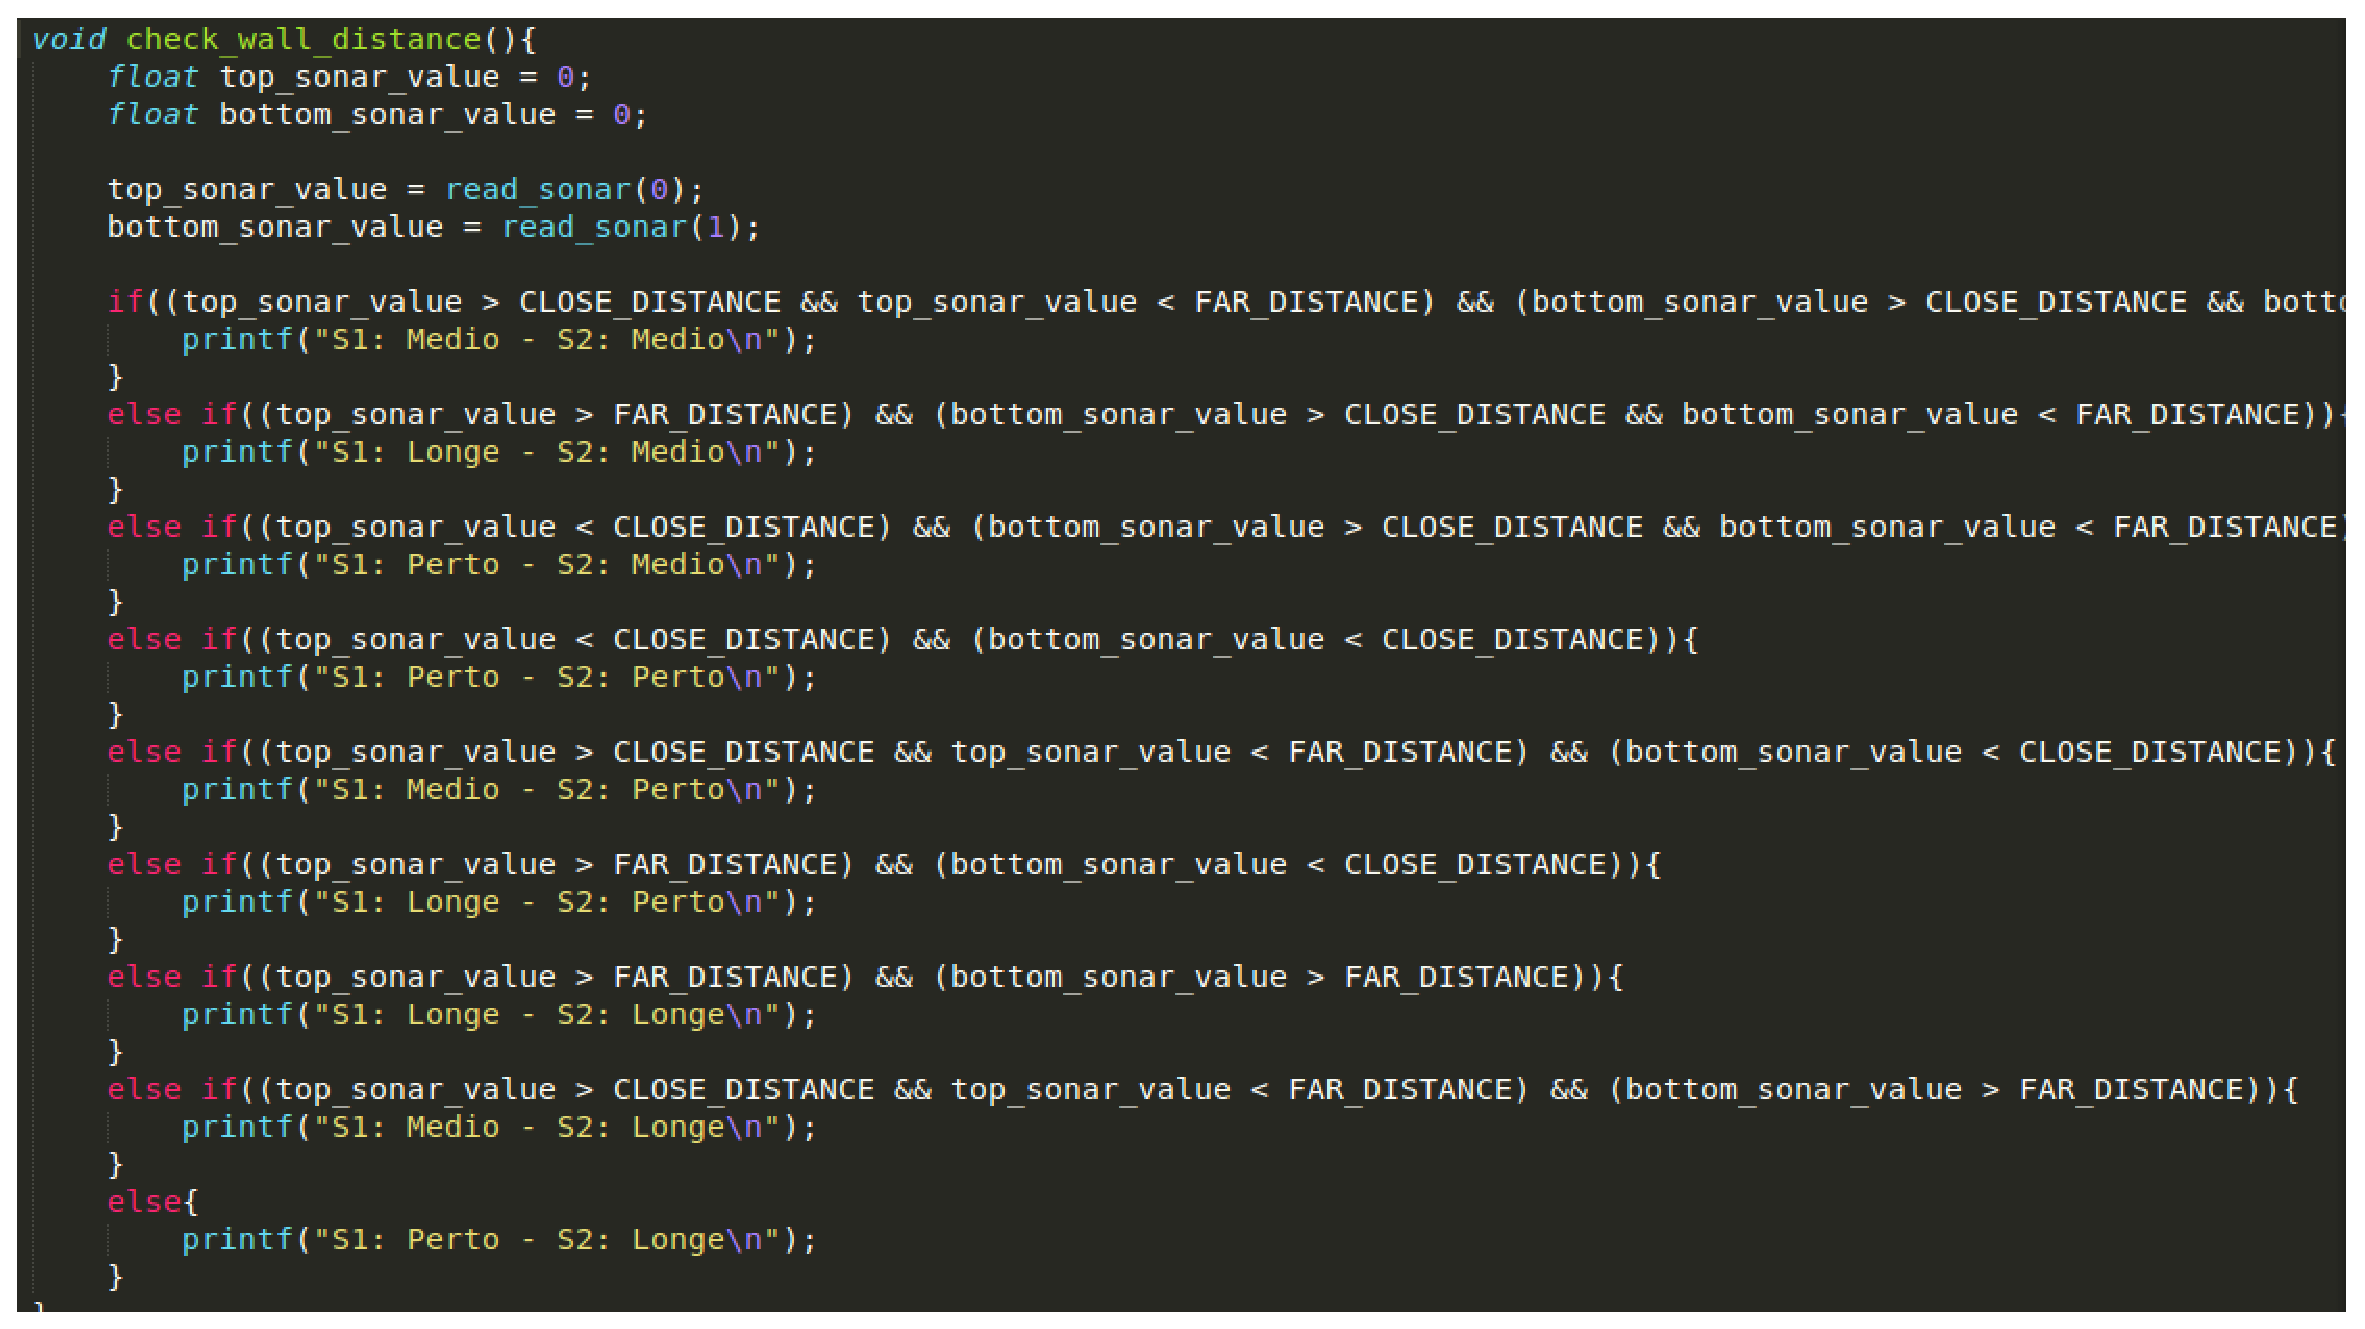
\includegraphics[width=1\textwidth]{figuras/check_wall_distance.eps}
  \caption{\label{fig:check_wall_distance}Corpo do Método \textit{check\_wall\_distance}.}
  \end{center}
  \end{figure}

  As funções \textit{make\_first\_curve}, \textit{make\_second\_curve} e \textit{make\_big\_curve} ainda não
  foram implementadas.

  \subsection{Informações}

  \subsubsection{Unidade de Processamento}

  Para processamento das informações foi
  escolhida foi o Raspberry Pi B+,
  É uma unidade robusta que conta com o microprocessador
  BCM2835 da Broadcom, com clock de
  700MHz e modo de baixo consumo, uma GPU Dual Core VideoCore
  IV\textregistered, SDRAM de 512MB, 4 portas USB, 1 porta RJ45
  (Ethernet), 1 porta HDMI e 40 pinos para GPIO~\cite{raspref}

  Esta unidade terá um sistema operacional Linux embarcado, responsável
  por gerenciar o armazenamento dos dados obtidos pelos sensores e
  processar decisões do controle do veículo.

  \begin{figure}[!htbp]
  \begin{center}
  \includegraphics[width=.7\textwidth]{figuras/raspberry.eps}
  \caption{\label{fig:raspberry}Raspberry Pi B+.}
  \end{center}
  \end{figure}

  \paragraph{UART}
	Considerando a troca de informações entre as plataformas de controle e
	processamento (Arduino e Raspberry Pi) surge a necessidade de definir
	um protocolo de comunicação comum. Centenas de protocolos de comunicação
	são capazes de viabilizar essa troca de dados. Considerando a universalidade
	e disponibilidade de recursos de hardware, optou-se por utilizar um
	protocolo serial a partir do UART.

	Um UART (universal asynchronous receiver/transmitter) é um bloco de circuitos
	responsável pela implementação da comunicação serial. Essencialmente, o UART
	age como um intermediário entre interfaces paralelas e em série. Conforme a
	figura~\ref{fig:uart}, uma das extremidades do UART é um barramento de oito linhas de
	dados (mais alguns pinos de controle), a outra é composta pelos fios de
	transmissão e recepção em série (TX e RX).

	\begin{figure}[!htbp]
	\begin{center}
	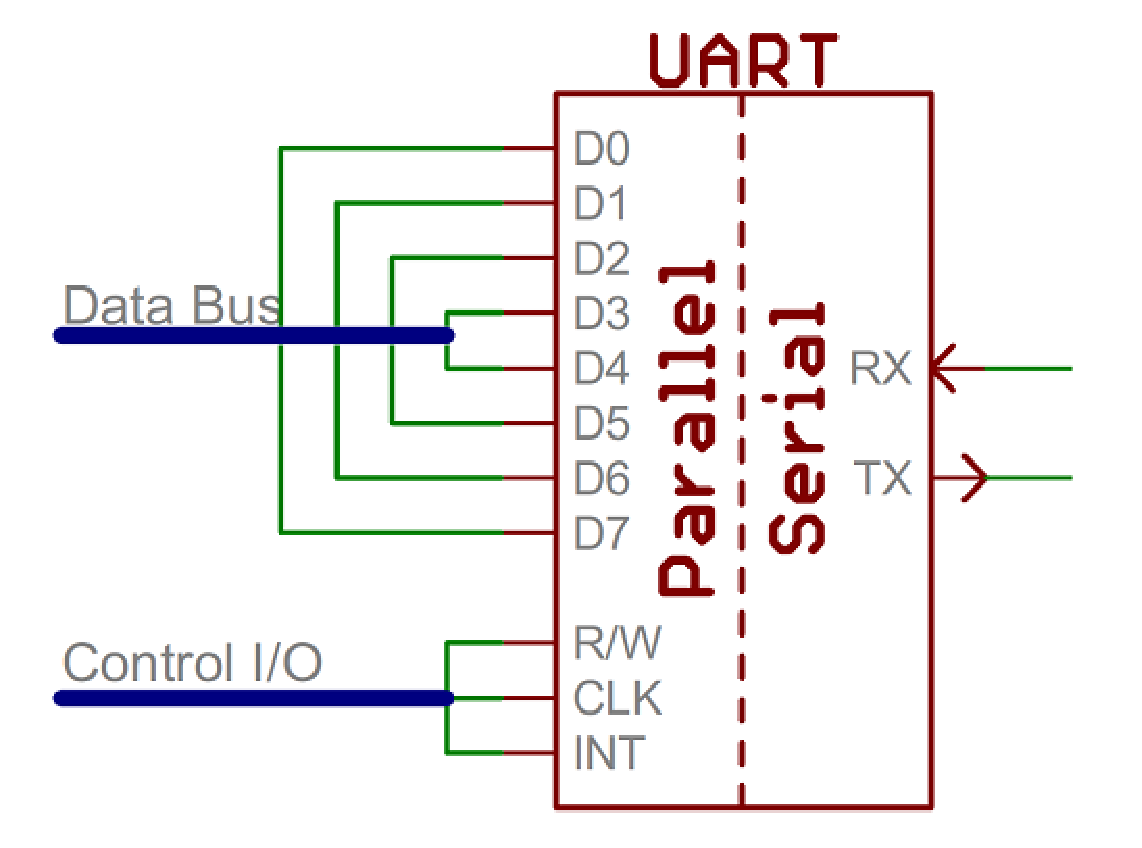
\includegraphics[width=.6\textwidth]{figuras/uart.eps}
	\caption{\label{fig:uart}Modelo simplificado da UART (fonte:~\citeonline{uartsparkfun}).}
	\end{center}
	\end{figure}

	Sistemas operacionais como o Linux contém bibliotecas nativas como a
	\texttt{termio.h} onde podem ser definidos o \textit{BAUD rate},
	segundos de espera entre bytes, números de bytes a ser lidos, etc.
	Essa é mais uma vantagem de utilizar tal protocolo de comunicação.

  \subsubsection{Armazenamento dos Dados}
  Os dados de configurações do veículo e resultados das medições serão armazenados
  em um cartão de memória inserido na Raspberry Pi, em um diretório definido.

  As medições serão gravadas em arquivos no formato CSV (\textit{Comma Separated Value}),
  dispostas em colunas na seguinte ordem: posição da medição
  em metros, umidade do solo, umidade relativa do ar e temperatura do
  ambiente.
  Os dados dispostos desta maneira facilitam o processamento e
  análise posterior, assim como sua apresentação gráfica para
  o operador.

  \begin{figure}[!htbp]
  \begin{center}
  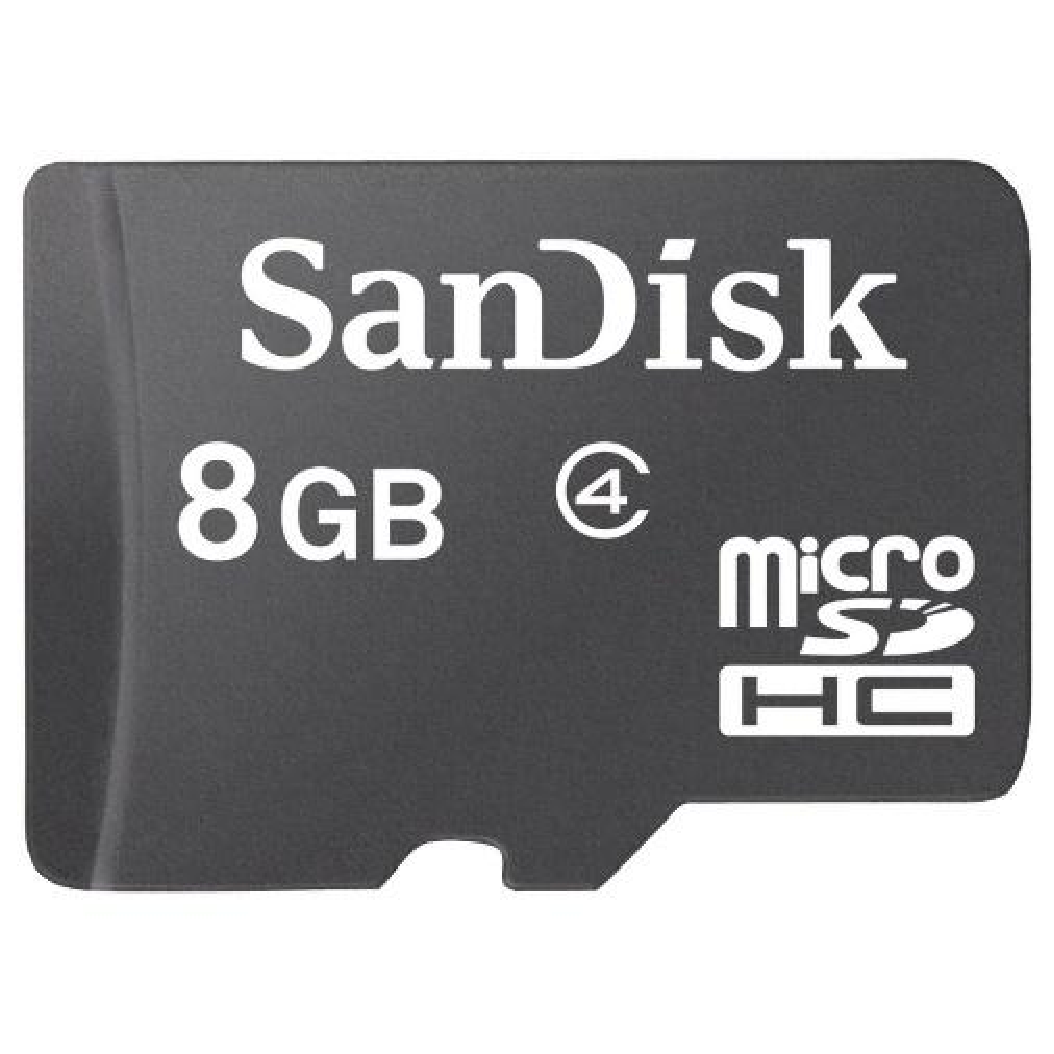
\includegraphics[width=.3\textwidth]{figuras/sdcard.eps}
  \caption{\label{fig:sdcard}Cartão de memória.}
  \end{center}
  \end{figure}

  Posteriormente, o acesso aos dados será feito através de uma conexão de  rede
  wireless entre um computador e a Raspberry. Para a comunicação  entre os
  dispositivos será utilizado o protocolo FTP, que é bastante utilizado para
  transferência de arquivos em uma rede.

  \subsubsection{Apresentação das Informações}

  Uma parte importante do projeto consiste na apresentação dos
  dados para o usuário encarregado pela gestão da lavoura. Para essa demanda,
  foi definido o desenvolvimento de uma aplicação web, utilizando
  o \textit{framework} Rails.

  A escolha de desenvolver utilizando-se essa linguagem junto a
  esse \textit{framework} foi feita com base na facilidade que essa
  tecnologia fornece para o desenvolvimento e com base na experiência
  da equipe responsável pelo desenvolvimento da aplicação, visto que
  todos os membros do grupo já possuem experiência com a tecnologia.

  Em concordância com os requisitos estabelecidos, essa aplicação
  permitirá o upload do arquivo CSV gerado pelo veículo, dentro de
  uma área restrita da aplicação, disponível apenas após a realização
  do login.
  Além da representação gráfica, o gestor da lavoura poderá obter
  esses dados em formato de relatório, sendo permitida sua
  exportação para um arquivo PDF (Portable Document Format).

  Após a obtenção dos dados, o usuário possuirá a opção de visualiza-los de forma gráfica, sendo que esta visualização se dará
  com base em um mapa de calor (\textit{heatmap}), conforme a figura \ref{fig:heatmap} representa, para uma melhor representação da lavoura.

  O conceito dos mapas de calor é baseado na representação de diversos pontos sobrepostos em um mapa, sendo que quanto mais pontos
  forem existentes em uma mesma posição, uma coloração mais forte será atribuída, por isso ganhando essa denominação.

  Para a implementação dos mapas de calor no contexto deste projeto, foi utilizada a API (\textit{Application Programming Interface})
  do Google Maps. Essa API permite acesso as imagens dos mapas e a posterior aplicação de uma camada com os pontos do mapa de calor.

  \begin{figure}[!htbp]
  \begin{center}
  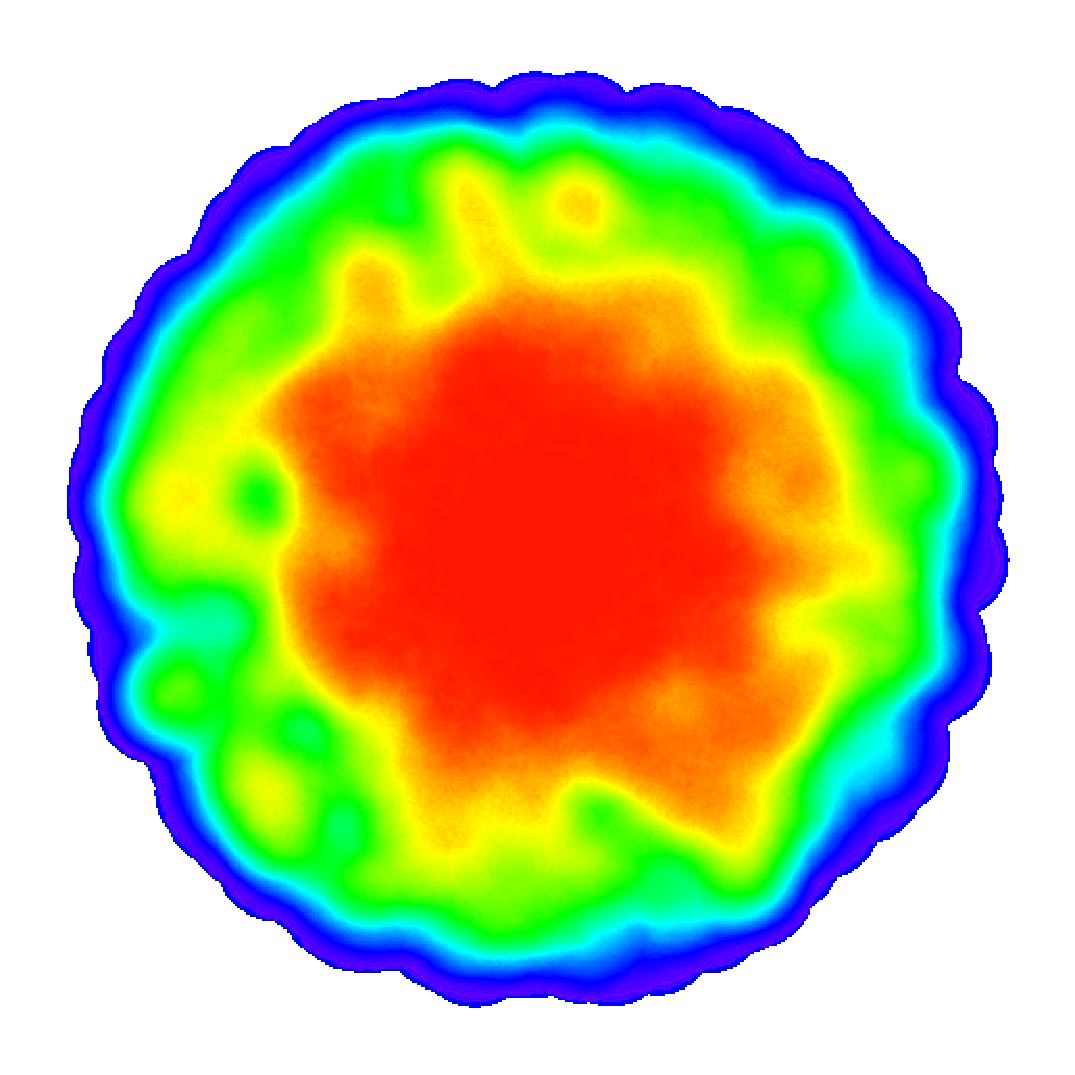
\includegraphics[width=.5\textwidth]{figuras/heatmap.eps}
  \caption{\label{fig:heatmap}Exemplo de mapa de calor.}
  \end{center}
  \end{figure}
